\documentclass{article}
\usepackage{hyperref}
\usepackage[procnames]{listings}
\usepackage{color}
\title{Assignment 2}
\date{2016-02-10}
\author{Tarek Fouda}
\usepackage[pdftex]{graphicx}
\usepackage{listings}
\usepackage{alltt}


\definecolor{dkgreen}{rgb}{0,0.6,0}
\definecolor{gray}{rgb}{0.5,0.5,0.5}
\definecolor{mauve}{rgb}{0.58,0,0.82}

\lstset{
	basicstyle=\footnotesize,
	breaklines=true,
}

\begin{document}
  \maketitle
\section{Introduction}
This report explains how I managed to solve Assignment 2 in Web Science class which is due 02/11/2016. It is mainly consisted of three Questions. Will show my approaches and implementation in each of the three Questions.

\section{Problem 1- Extracting 1000 unique URLs from Twitter newsfeed}

\subsection{My approach}

Baiscally I had to create a twitter account which I already have, also I had to register for a new twitter application to get the Consumer key, Consumer secret key, Key token and secret key token.

These variables allow you to use a Twitter python  API, by just inserting these variables in your code. You would be able to, for example, Post a status from python code.
But in this part of the assignment we are required to 1000 unique links from the newsfeed or even from someone's profile on Twitter.

I downloaded python-Twitter API from Github \url{https://github.com/ideoforms/python-twitter-examples}. It has a lot of python files which do specific tasks, for example twitter-list-retweets.py which lists all the retweets received on a specific tweet. What we only care about is extracting links.
\begin{figure}
\centering
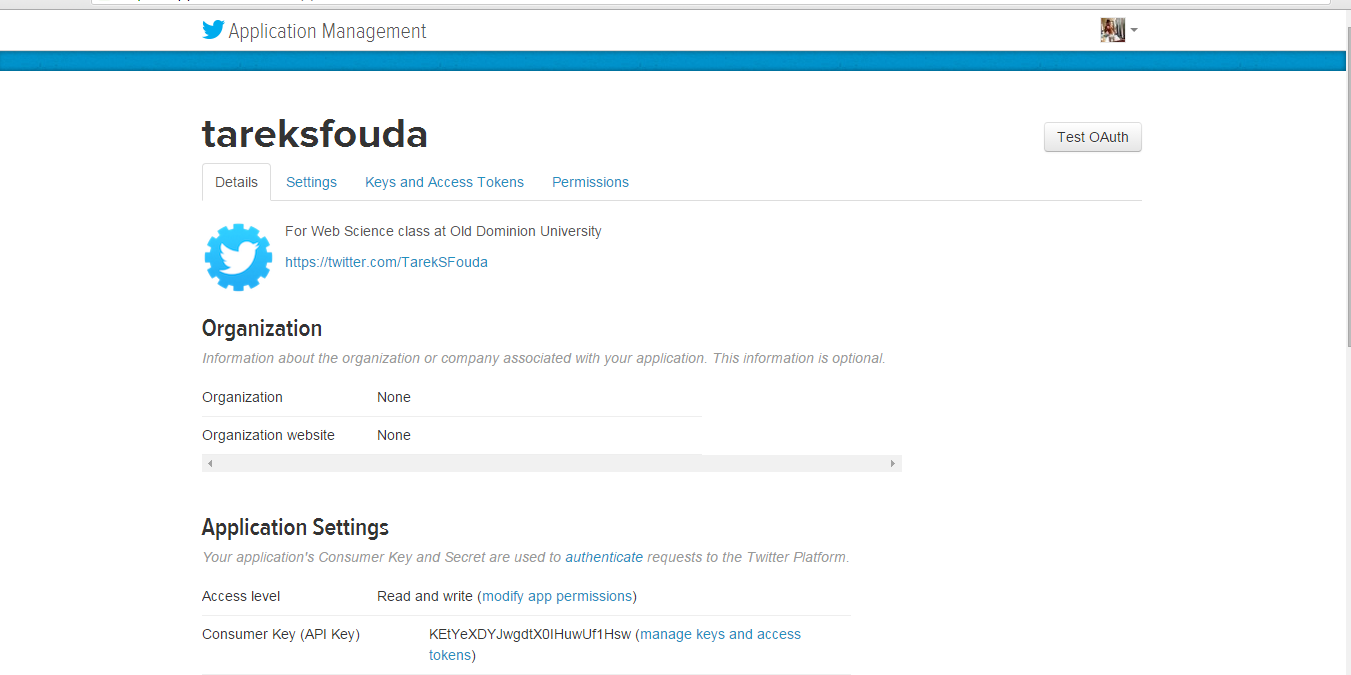
\includegraphics[scale=0.35]{appstwitterQ1.png}
\caption{Twitter app}
\label{fig:appstwitterQ1}
\end{figure}
Creating a twitter application was the first thing I should do, following the steps on \url{https://github.com/ideoforms/python-twitter-examples} made me capable of creating a twitter app and now I can go to the config.py file and Type in my accesscode and secret keys Tokens as follows:

\lstinputlisting[language=Python,frame=single,caption={Config.py},label=lst:q2code1,captionpos=b,numbers=left,
numberstyle=\tiny\color{gray},
  keywordstyle=\color{blue},
  commentstyle=\color{dkgreen},
  stringstyle=\color{mauve},showspaces=false,showstringspaces=false,basicstyle=\footnotesize]{config.py}
\begin{figure}
\centering
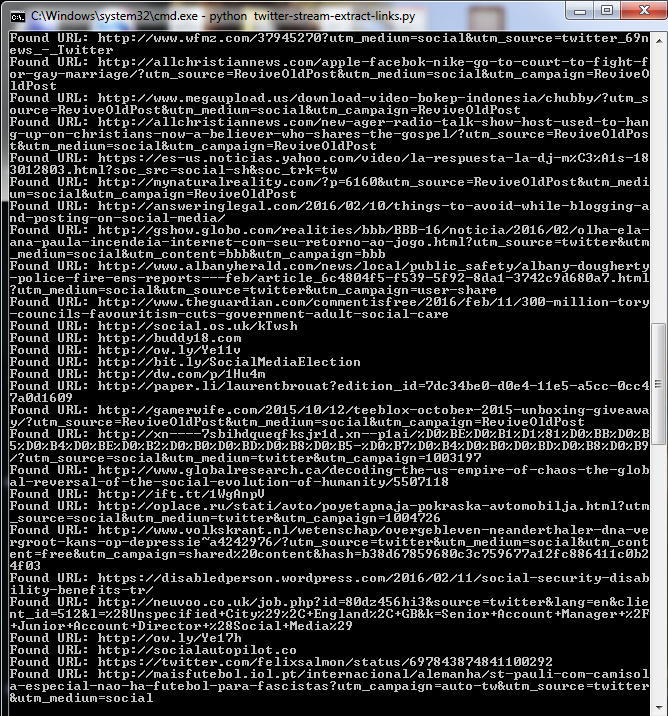
\includegraphics[scale=0.75]{cmd-Q1.png}
\caption{Printing the unique URLS}
\label{fig:cmd-Q1}
\end{figure}
The actual code that should be implemented lies in twitter-stream-extract-links.py.
\lstinputlisting[language=Python,frame=single,caption={Python program for extracting links from my Twitter newsfeed},label=lst:q2code1,captionpos=b,numbers=left,
numberstyle=\tiny\color{gray},
  keywordstyle=\color{blue},
  commentstyle=\color{dkgreen},
  stringstyle=\color{mauve},showspaces=false,showstringspaces=false,basicstyle=\footnotesize]{twitter-stream-extract-links.py}

as shown above the code loops to find all Tweets found in my newsfeed, we basically put all the expanded URLS that are found in Twitter feed in a list. How can we assure that the link is Unique and not repetetive? This check happens in line 18. Tha if condition statement does not put the URL in the list unless it is unique.
I kept all the llist in a text file by writing every unique URL in a text file called urls.txt as shown in line 20.

\subsection{The list}
Listing the 1000 links I got will make this report unofficial so I refered to the text file I created that has all the URLS which is named urls.txt


\section{Problem number 2 - Finding TimeMaps and Histogram}

In this problem, it was required to download the TimeMaps for each link I got in the first problem. I basically downloaded a python code from Github \url{github.com/jocll}. The file is called timemap.py and it simply takes a url as an argument and print out the TimeMaps and mementos for this URL.
But in my situation, I need to find the TimeMaps for all URLS I have, so I had to amend the code to be able to read the URLs from the urls.txt and loop to perform getting Time Maps for all the URLs I have. the code was as follows:

\lstinputlisting[language=Python,frame=single,caption={Time map python code},label=lst:q2code1,captionpos=b,numbers=left,
numberstyle=\tiny\color{gray},
  keywordstyle=\color{blue},
  commentstyle=\color{dkgreen},
  stringstyle=\color{mauve},showspaces=false,showstringspaces=false,basicstyle=\footnotesize]{timemap.py}

\begin{figure}
\centering
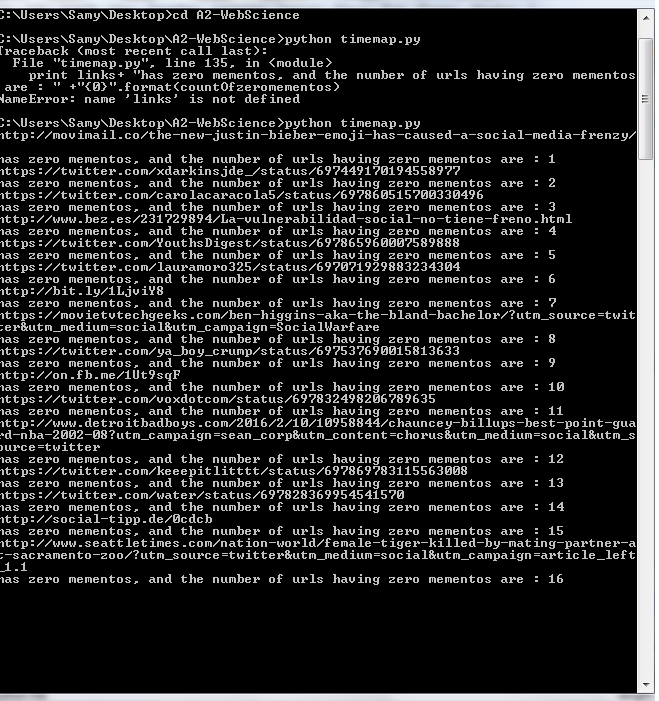
\includegraphics[scale=0.75]{q2mementosnumbers.png}
\caption{A samplefor the URLs with their mementos}
\label{fig:q2mementosnumbers}
\end{figure}

In line 116, we Opened the text file to read all the URL's in there, and we looped on each URL to count the Time Maps, and if a 404 message is printed, then the corresponding link has zero mementos. that was kept track of in the exception part, from line 133.

Keeping in mind I kept track of the numbers of the links that have zero mementos, in line 134 of the code.

This a sampleof the command prompt upon running the amended code:


We were required also to draw a Histogram to show the number of URLs and the mementos, for example 100 URL's having 0 mementos and 200 URL's having 1 memento and so on.
\newpage
\section{Problem number 3 Estimate the age of URLs}

Finally the last part of the assignment was to estimate the age (Creation date) of each of the URLs, I downloaded Carbon date API and in the local.py file it was easy to pass a URL as an argument and print out its carbon date, but What is required is calculating the age of all URLs, so I implemented a function in cdate.py file to call the local.py downloaded within the Carbondate API, and pass every URL as an argument in a loop. so the final code will calculate the carbon date for all URLS. Then I copied and pasted the output in a file which to be read by a function in Python called q3.py which basically reads all the text file and disregard everything other than the URL and the corresponding Creation date.
\newpage
\lstinputlisting[language=Python,frame=single,caption={q3.py},label=lst:q2code1,captionpos=b,numbers=left,
numberstyle=\tiny\color{gray},
  keywordstyle=\color{blue},
  commentstyle=\color{dkgreen},
  stringstyle=\color{mauve},showspaces=false,showstringspaces=false,basicstyle=\footnotesize]{Q3/q3.py}

Basically I put all the output in a text file and read it in a list, then as soon as I find a creation date, I print it out along with the corresponding URL, Keeping in mind I do not print out the URLs that do not have a creation date. Here is a figure which shows a sampleof the output upon calling q3.py :
\begin{figure}
\centering
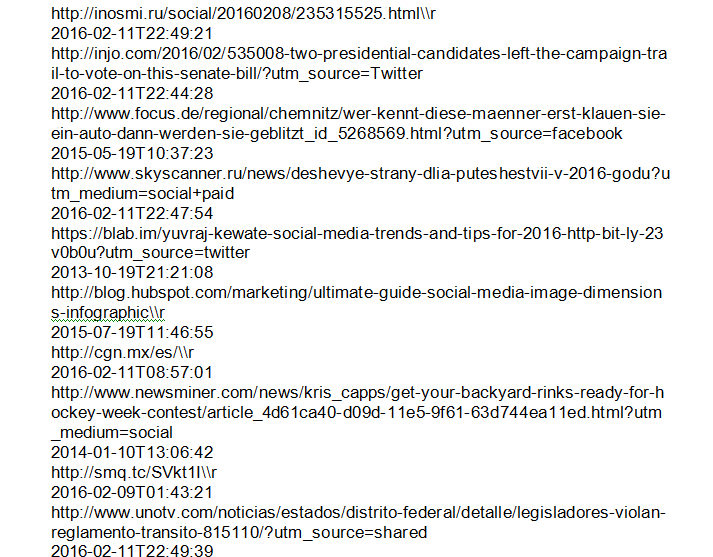
\includegraphics[scale=0.75]{q3fig.png}
\caption{A samplefor the output from q3.py, URLs and their age}
\label{fig:q3fig.png}
\end{figure}

The following figure represents a graph between The Creation Dates and mementos for only the links that have both mementos and creation dates. X axis represents the age in Years and Y- axis represent the corresponding mementos. The Graph is based on  the Output file shown above and Figure 3 which states the mementos for all URLs.

\begin{figure}
\centering
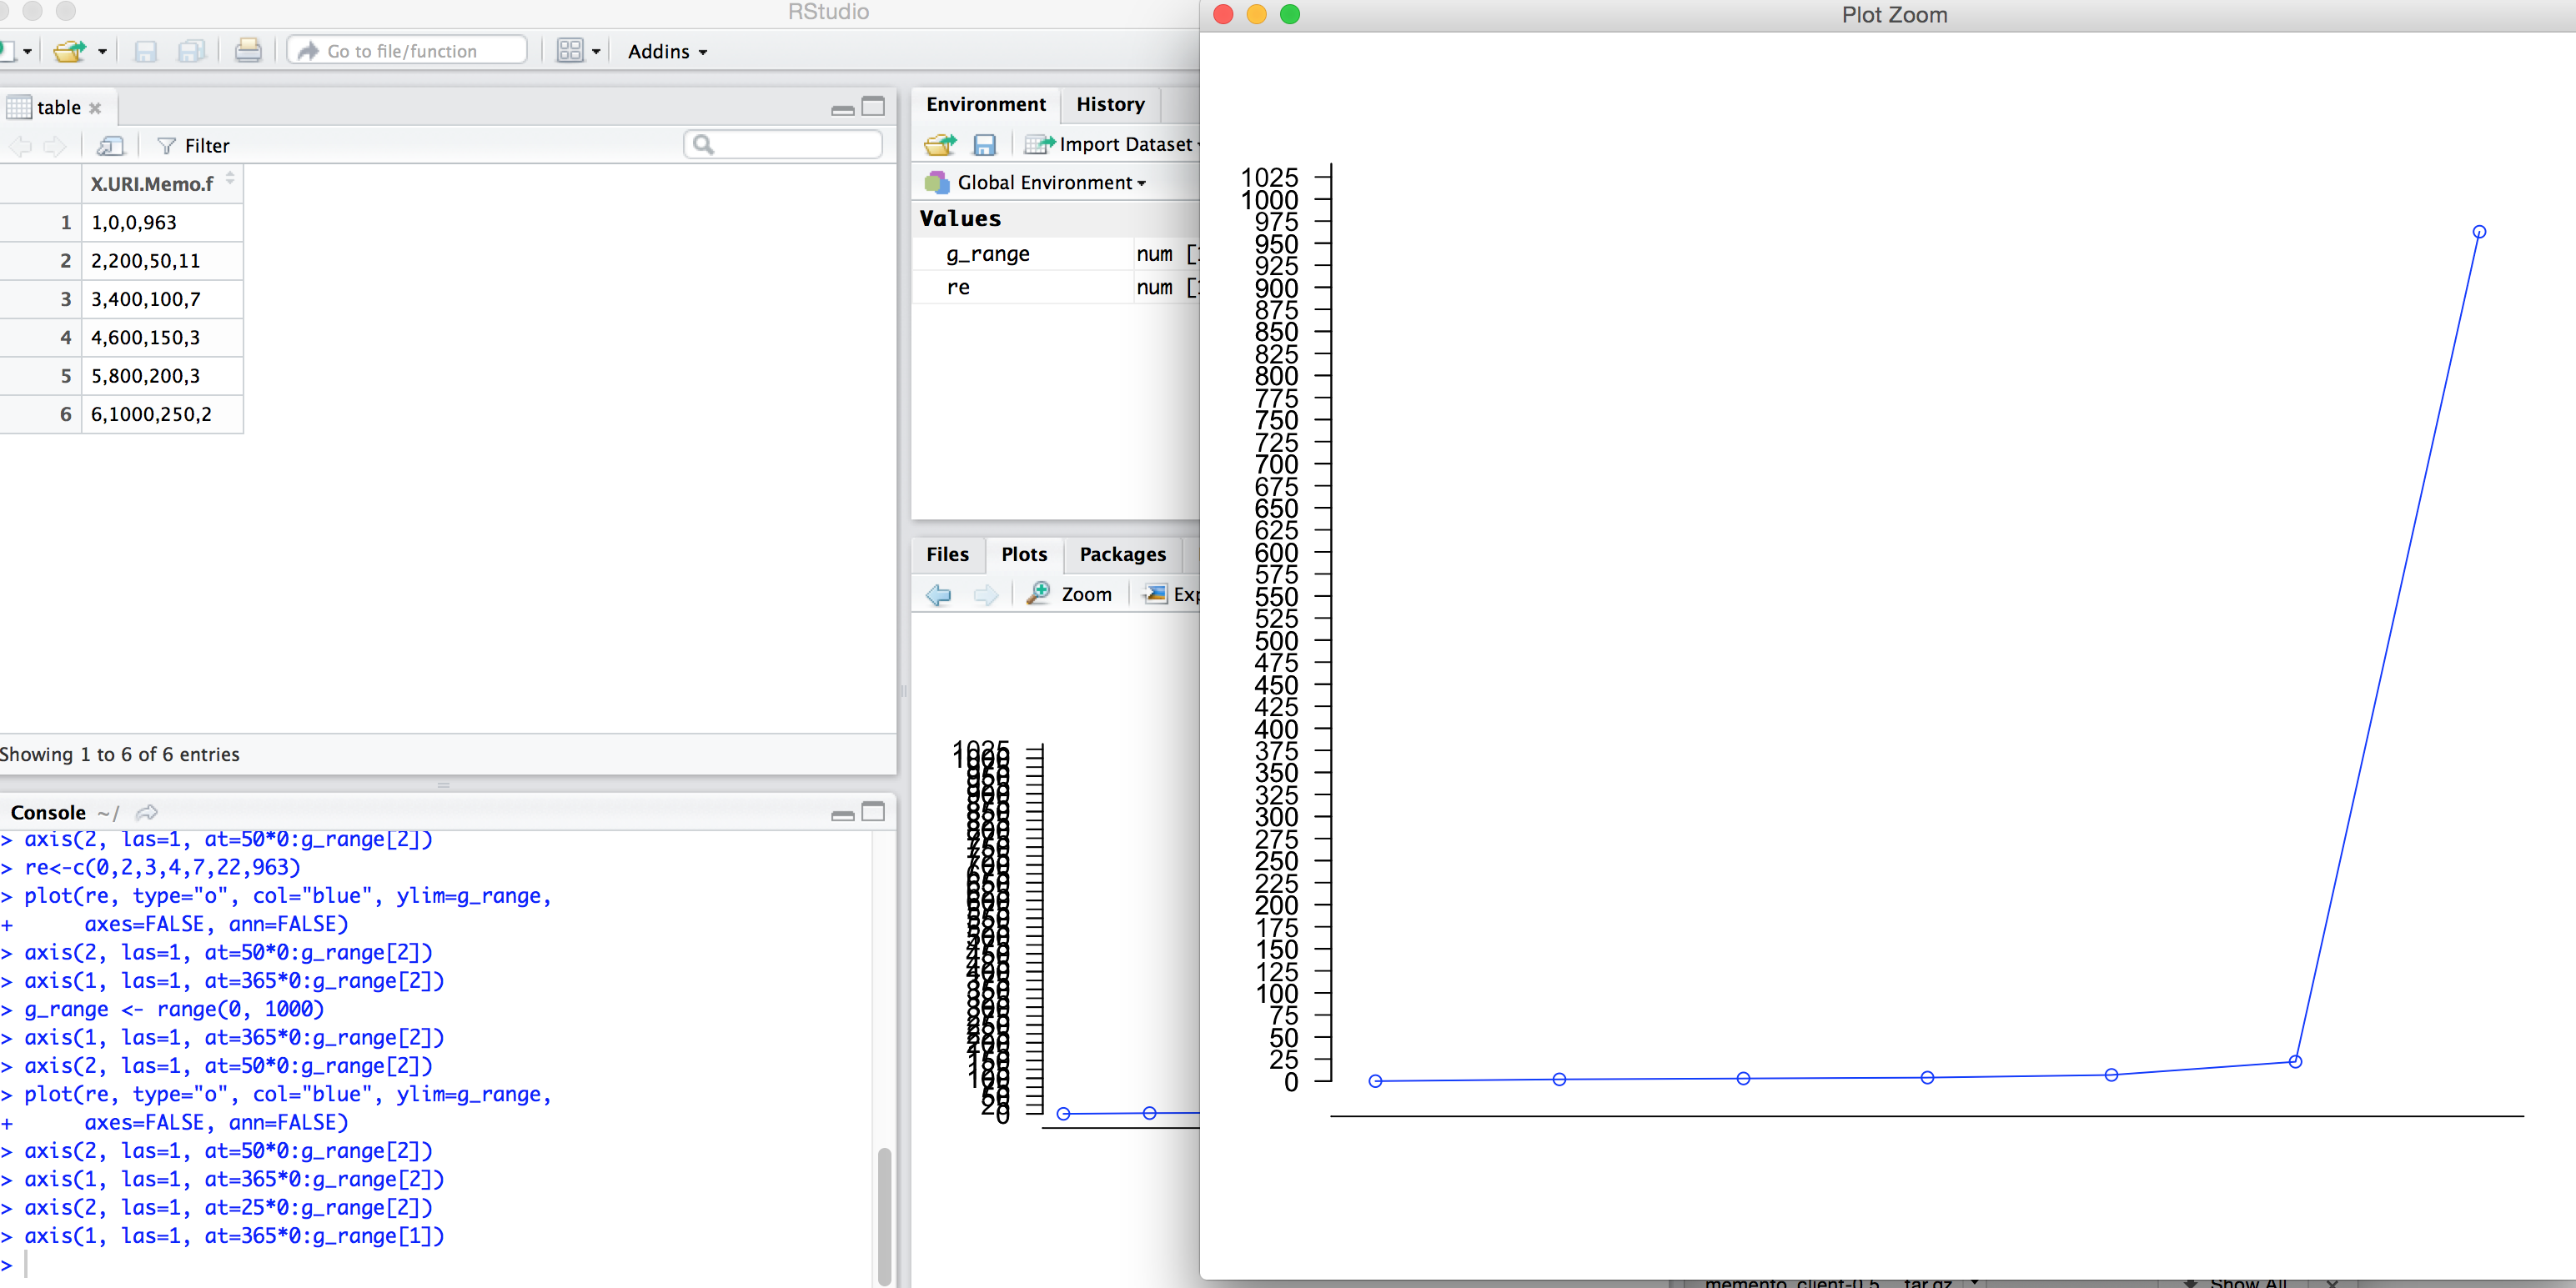
\includegraphics[scale=0.15]{graph.png}
\caption{A samplefor the output from q3.py, URLs and their age}
\label{fig:graph.png}
\end{figure}
\end{document}